\chapter{M\'etodo Matricial para Solu\c{c}\~ao de EDO's}

Este cap\'itulo trata do estudo do m\'etodo matricial para analisar a propaga\c{c}\~ao de ondas em subsuperf\'icie terrestre, conforme estruturado em \cite{Ursin-1983}. Gra\c{c}as a similaridade matem\'atica entre sistemas de EDP's eletromagn\'eticas (Maxwell) e sistemas de EDP's el\'asticas (Lamè), podemos dar um desenvolvimento unificado para esses sistemas. Utilizamos um conjunto de transformadas e mudan\c{c}a de eixos coordenados para dividir esses dois sistemas de EDP's em quatro sistemas de EDO's escritos em forma matricial, onde as vari\'aveis dependentes estejam em fun\c{c}\~ao apenas da profundidade e da frequ\^encia temporal. Os coeficientes desses sistemas de EDO's podem ser reunidos numa matriz $M$ de dimens\~ao $2n\times 2n$, a qual pode ser particionada em quatro submatrizes de dimens\~ao $n\times n$, e \'e usada como o ponto de partida para o estudo da propaga\c{c}\~ao de ondas em subsuperf\'icie.  

As propriedades de simetria da matriz $M$ nos permitem separar o campo de ondas em ascendentes e descendentes atrav\'es de uma decomposi\c{c}\~ao em autovetores. Essas propriedades nos permitem tamb\'em deduzir caracter\'isticas invariantes da propaga\c{c}\~ao, onde uma dessas caracter\'isticas \'e v\'alida apenas para meios de baixa dissipa\c{c}\~ao de ondas e correspondem \`a conserva\c{c}\~ao de energia. A matriz de propaga\c{c}\~ao de ondas pode ser computada para camadas homog\^eneas ou n\~ao, atrav\'es de um m\'etodo relativamente simples. Dado o vetor de ondas na camada superficial, podemos calcular seu valor para qualquer camada usando a matriz de propaga\c{c}\~ao.

A propaga\c{c}\~ao de ondas em meios estratificados produz fen\^omenos de transmiss\~ao e reflex\~ao de ondas. Dadas as dedu\c{c}\~oes das matrizes de transmiss\~ao e reflex\~ao, podemos relacion\'a-las com a matriz de propaga\c{c}\~ao, bem como deduzir propriedades de simetrias para essas matrizes atrav\'es das caracter\'isticas invariantes da propaga\c{c}\~ao. Podemos ainda deduzir as matrizes de transmiss\~ao e reflex\~ao modificadas para pilha de camadas limitadas superiormente por uma superf\'icie livre.

\section{Caracter\'isticas das Equa\c{c}\~oes na Forma Matricial de Ursin}

%Sendo $\mathbf{x}=(x,y,z)^{\top}$ o espa\c{c}o $\mathbb{R}^3$ e aplicando as tranformadas de Fourier direta e inversa na forma
%\begin{align*}
%F(\omega,k_1,k_2,z) &= \iiint_{-\infty}^{\infty}f(t,x,y,z)\,e^{i\omega t-ik_1x-ik_2y}dt\,dxdy\\\\
%f(t,x,y,z) &= \left(\frac{1}{2\,\pi}\right)^3\,\iiint_{-\infty}^{\infty}F(\omega,k_1,k_2,z)\,e^{-i\omega t+ik_1x+ik_2y}d\omega\,dk_1dk_2\,,
%\end{align*}
%podemos escrever um conjunto de EDP's que descevem a propaga\c{c}\~ao de ondas sismomagn\'eticas em camadas horizontais da subsuperf\'icie terrestre somente em fun\c{c}\~ao da profundidade $z$. 
%
%A t\'itulo de exemplo, tanto as EDP's de Maxwell para o eletromagnetismo
%\begin{align}\label{eq.faraday_ampere}\nonumber
%\nabla\times\mathbf{E}&=-\frac{\partial}{\partial t}\mathbf{B}\\\\\nonumber
%\nabla\times\mathbf{H}&=\sigma\mathbf{E}+\frac{\partial}{\partial t}\mathbf{D}+\mathbf{G}\,,
%\end{align}
%como as EDP's el\'asticas
%\begin{align}\label{eq.cauchy_hooke}\nonumber
%\rho\frac{\partial^2 \mathbf{U}}{\partial t^2}&=\nabla\cdot\tau+\mathbf{F}\\\\\nonumber
%\tau&=\lambda\nabla\cdot \mathbf{U}\cdot I + \mu(\nabla \mathbf{U}+\nabla \mathbf{U}^*)\,,
%\end{align}
%podem ser escritas no formato matricial apresentado por Ursin, ou seja, 
\'E poss\'ivel utilizar o m\'etodo matricial no formato preconizado por \cite{Ursin-1983} para resolver sistemas de EDO's desde que se possa escrever tal sistema como
\begin{align}\label{eq.matricial}
\frac{\partial\,\mathbf{\Phi}^{(m)}}{\partial\,z} &= -\,i\,\omega\,M^{(m)}\,\mathbf{\Phi}^{(m)}+\mathbf{S}^{(m)},\quad\text{com}\quad m\,\in\mathbb{N},
\end{align}
%\begin{bmatrix}
%\mathbf{\Phi_1}\\
%\mathbf{\Phi_2}	
%\end{bmatrix}\,,
onde $\mathbf{S}^{(m)}$ \'e um vetor de fonte de onda s\'ismica de dimens\~ao $2\,n_m$ e as matrizes $M^{(m)}_{2\,n_m\times2\,n_m}$ t\^em o formato
\begin{equation}\label{eq.matriz_M}
M^{(m)}
=
\begin{pmatrix}
\mathbf{0}&M_1^{(m)}\\
M_2^{(m)}&\mathbf{0}
\end{pmatrix},
\end{equation}
onde $M_1^{(m)}$ e $M_2^{(m)}$ s\~ao submatrizes sim\'etricas de dimens\~ao $n_m\times n_m$.

A equa\c{c}\~ao \ref{eq.matricial} tem as seguintes caracter\'isticas:
\begin{itemize}
\item $M^{(m)}_{2\,n\times2\,n}$ \'e uma matriz que pode ser particionada em quatro submatrizes $n\times n$, com submatrizes de zeros na diagonal principal e submatrizes sim\'etricas $M_1^{(m)}$ e $M_2^{(m)}$ na diagonal secund\'aria. As componentes de $M_1^{(m)}$ e $M_2^{(m)}$ s\~ao fun\c{c}\~oes dos par\^ametros das EDP's que est\~ao sendo trabalhadas, s\~ao fun\c{c}\~oes tamb\'em de $z$ e do vetor real de vagarosidade $\pmb{\gamma}=\frac{\mathbf{k}}{\omega}$. Para meios de baixa dissipa\c{c}\~ao das ondas, as matrizes $M_1^{(m)}$ e $M_2^{(m)}$ s\~ao reais; 
\item O vetor de onda $\mathbf{\Phi}^{(m)}$ tem dimens\~ao $2n\times1$ e \'e particionado em dois vetores $\mathbf{\Phi}^{(m)}_1$ e $\mathbf{\Phi}^{(m)}_2$ com dimens\~ao $n\times1$ . As componentes do vetor de onda s\~ao escolhidas de forma que $\mathbf{\Phi}^{(m)}$ seja cont\'inuo atrav\'es das fronteiras entre duas camadas;
\item  Para ondas el\'asticas, metade das componentes de $\mathbf{\Phi}^{(m)}$ s\~ao zeros na superf\'icie livre, ou seja, existe uma matriz de permuta\c{c}\~ao $T_{2n\times2n}$ onde $T^{-1}=T^\top$ e tal que
\begin{equation*}
\begin{bmatrix}
\mathbf{V}_1(\mathbf{0})\\
\mathbf{0}
\end{bmatrix}
=T\,\mathbf{\Phi}^{(m)}\quad\text{quando}\quad z = 0\,;
\end{equation*}
%\item As componentes do vetor de onda $\mathbf{\Phi}^{(m)}$ s\~ao escolhidas de forma que o fluxo de energia na dire\c{c}\~ao $z$ seja dado por
%\begin{equation*}
%J=-\frac{1}{4}(\mathbf{\Phi}_1^{(m)\,H}\mathbf{\Phi}^{(m)}_2+\mathbf{\Phi}_2^{(m)\,H}\mathbf{\Phi}^{(m)}_1)=-\frac{1}{4}\mathbf{\Phi}^{(m)\,H}\,M_0\mathbf{\Phi}^{(m)}\,,
%\end{equation*}
%onde $H$ denota complexo conjugado transposto,
%\begin{equation*}
%M_0=
%\begin{bmatrix}
%0_{n\times n}&I\\
%I&0_{n\times n}
%\end{bmatrix}
%\end{equation*}
%e $I$ \'e uma matriz identidade $n\times n$.
\end{itemize}

O m\'etodo a seguir \'e aplicado em equa\c{c}\~oes escritas no formato matricial \ref{eq.matricial}, com ondas se propagando numa pilha de camadas homog\^eneas e assumimos que os par\^ametros das equa\c{c}\~oes s\~ao fun\c{c}\~oes cont\'inuas no interior de cada camada e que dependem apenas da profundidade $z$. O modelo inclui pilha de camadas homog\^eneas com par\^ametros constantes por camada e consideramos o eixo $z$ como sendo positivo no sentido descendente.

\section{Diagonaliza\c{c}\~ao}\label{sec.diagonalizacao}
Considere matrizes $M$ conforme a equa\c{c}\~ao \ref{eq.matriz_M}, onde por simplicidade de escrita n\~ao usaremos o sobrescrito $m$. Vamos aplicar nesta matriz um procedimento de diagonaliza\c{c}\~ao que pode ser encontrado em trabalhos como \cite{Ursin-1983}, \cite{White_Zhou_2006} e \cite{Azeredo_2013}.

Seja $(\mathbf{a}_m,\,\mathbf{b}_m)^\top$ seja um autovetor da matriz $M$ associado ao autovalor $q_m$, com $m=1,...,n$, assim
\begin{equation}
\begin{pmatrix}
0_{n\times n}&M_1\\
M_2&0_{n\times n}
\end{pmatrix}
\begin{pmatrix}
\mathbf{a}_m\\
\mathbf{b}_m
\end{pmatrix}
=
q_m\,
\begin{pmatrix}
\mathbf{a}_m\\
\mathbf{b}_m
\end{pmatrix}.
\end{equation}
Ou seja, 
\begin{equation}\label{eq.M1_b}
M_1\mathbf{b}_m=q_m\,\mathbf{a}_m 
\end{equation}
e
\begin{equation}\label{eq.M2_a}
M_2\mathbf{a}_m=q_m\,\mathbf{b}_m. 
\end{equation}
Multiplicando \ref{eq.M1_b} pela esquerda por $M_2$ e substituindo \ref{eq.M2_a}, temos
\begin{equation}\label{eq.m2m1bm}
M_2M_1\mathbf{b}_m=q_m^2\mathbf{b}_m.
\end{equation} 
Analogamente, multiplicando \ref{eq.M2_a} pela esquerda por $M_1$ substituindo \ref{eq.M1_b}, temos 
\begin{equation}\label{eq.m1m2am}
M_1M_2\mathbf{a}_m=q_m^2\mathbf{a}_m.
\end{equation}
Desta forma, $\mathbf{a}_m$ \'e um autovetor associado \`a matriz $M_1M_2$, e $\mathbf{b}_m$ \'e um autovetor associado \`a matriz $M_2M_1$. 

Como estamos assumindo que $M_1$ e $M_2$ s\~ao sim\'etricas, partindo da equa\c{c}\~ao \ref{eq.m2m1bm} e usando a equa\c{c}\~ao \ref{eq.m1m2am}, temos
\begin{align*}
q_m^2\mathbf{b}_m&=M_2M_1\mathbf{b}_m\\
q_m^2\mathbf{a}_j^\top\mathbf{b}_m&=\mathbf{a}_j^\top M_2M_1\mathbf{b}_m\\
&=\mathbf{b}_m^\top M_1M_2\mathbf{a}_j\\
&=q_j^2\mathbf{a}_j^\top\mathbf{b}_m.
\end{align*}
Isolando $\mathbf{a}_j^\top\mathbf{b}_m$ na \'ultima igualdade acima, temos que 
\begin{empheq}[left={\mathbf{a}_j^\top\mathbf{b}_m=\empheqlbrace}]{align}\label{eq.ajTbm}\nonumber
0\,,&\quad\text{se}\quad m\neq j\\\\\nonumber
\alpha_{j,m}\,,&\quad\text{se}\quad m=j,
\end{empheq}
onde $\alpha$ \'e um valor indeterminado.

Vamos definir a matriz $L_1$ de dimens\~ao $n\times n$ onde cuja $m$-\'esima coluna \'e dada por $\mathbf{a}_m$, e a matriz $L_2$ tamb\'em de dimens\~ao $n\times n$ cuja $m$-\'esima coluna \'e dada por $\mathbf{b}_m$. Assim, podemos reescrever as equa\c{c}\~oes \ref{eq.M1_b} e \ref{eq.M2_a}, respectivamente, como
\begin{align}\label{eq.m1l2}
M_1L_2&=L_1\Lambda\\\label{eq.m2l1}
M_2L_1&=L_2\Lambda,
\end{align}
onde a matriz $\Lambda_{n\times n}$ \'e a matriz diagonal dos autovalores. Observe que podemos trabalhar com as equa\c{c}\~oes normalizadas tomando $\alpha_{j,m}=1$ na equa\c{c}\~ao \ref{eq.ajTbm}, que passa a definir o s\'imbolo \textit{Delta de Kroneker}\footnote{Nos abstivemos de usar o caracter grego $\delta$ na equa\c{c}\~ao \ref{eq.ajTbm} por este j\'a definir a fun\c{c}\~ao Delta de Dirac em nosso escopo.}, conforme \cite{lebedev_2003}. Assim, escrevemos as componentes de $\Lambda$ como $\Lambda_{j,m}=q_j\mathbf{a}_j^\top\mathbf{b}_m$. Observe ainda que, deste modo, a equa\c{c}\~ao \ref{eq.ajTbm} define a matriz identidade $I_{n\times n}$, a qual podemos usar para mostrar que
\begin{align}\label{eq.l1l2}
L_1^{-1}&=L_2^\top\\\label{eq.l2l1}
L_2^{-1}&=L_1^\top.
\end{align}
Multiplicando pela direita as equa\c{c}\~oes \ref{eq.m1l2} e \ref{eq.m2l1} respectivamente por $L_2^{-1}$ e $L_1^{-1}$, e substituindo as equa\c{c}\~oes \ref{eq.l1l2} e \ref{eq.l2l1}, temos
\begin{align}
M_1&=L_1\Lambda L_1^\top\\
M_2&=L_2\Lambda L_2^\top.
\end{align}
Definindo a matriz $L_{2\,n\times 2\,n}$ como
\begin{equation}\label{eq.matriz_L}
L=\frac{1}{\sqrt{2}}
\begin{pmatrix}
L_1&L_1\\
L_2&-L_2
\end{pmatrix},
\end{equation}
e a matriz $\tilde{\Lambda}$ como
\begin{equation}\label{eq.tildeLambda}
\tilde{\Lambda}=
\begin{pmatrix}
\Lambda&0\\
0&-\Lambda
\end{pmatrix},
\end{equation}
podemos deduzir que
\begin{equation}\label{eq.L^-1}
L^{-1}=\frac{1}{\sqrt{2}}
\begin{pmatrix}
L_2^\top&L_1^\top\\
L_2^\top&-L_1^\top
\end{pmatrix}
\end{equation}
e
\begin{equation}\label{eq.m_semelhante_lambda}
M=L\,\tilde{\Lambda}\,L^{-1}.
\end{equation}

\section{Solu\c{c}\~ao de EDO's na Aus\^encia de Fonte}\label{sec.ausencia_fonte}

Vamos determinar inicialmente a solu\c{c}\~ao de EDO's  considerando o meio homog\^eneo e livre de fonte de onda s\'ismica. Ap\'os a diagonaliza\c{c}\~ao das equa\c{c}\~oes, podemos aplicar um m\'etodo utilizado por alguns autores como \cite{Ursin-1983}, \cite{Azeredo_2013}, \cite{White_Zhou_2006}, \cite{miranda_2016} entre outros, para determinar as solu\c{c}\~oes na aus\^encia de fonte. Esse mesmo m\'etodo pode ser utilizado para determinar as solu\c{c}\~oes na presen\c{c}a de fonte como veremos no cap\'itulo \ref{sec.presenca_fonte}. Aus\^encia de fonte significa que temos $\mathbf{S}^{(m)}=0$ na equa\c{c}\~ao \ref{eq.matricial}. A matriz ${M}^{(m)}$ possui entradas constantes por camada estratigr\'afica, as submatrizes na diagonal principal s\~ao nulas e as submatrizes na diagonal secund\'aria s\~ao sim\'etricas. 

\subsection{Ondas Ascendentes e Ondas Descendentes}

Vamos redefinir o vetor de ondas como
\begin{equation}\label{eq.Phi}
\mathbf{\Phi}=L\,\mathbf{\Psi}.
\end{equation}
Substituindo a equa\c{c}\~ao \ref{eq.Phi} na equa\c{c}\~ao \ref{eq.matricial}, temos
\begin{equation}\label{eq.matricial_sem_fonte}
\frac{\partial\,\mathbf{\Psi}}{\partial\,z} =-\,i\,\omega\,L^{-1}M\,L\,\mathbf{\Psi},
\end{equation}
onde o sobrescrito $m$ est\'a sendo omitido por quest\~ao de simplicidade.
De acordo com a equa\c{c}\~ao \ref{eq.m_semelhante_lambda}, temos que as matrizes $M$ e $\tilde{\Lambda}$ s\~ao semelhantes, assim
\begin{equation*}
\tilde{\Lambda}=L^{-1}M\,L.
\end{equation*}
Substituindo $\tilde{\Lambda}$ na equa\c{c}\~ao \ref{eq.matricial_sem_fonte}, temos
\begin{equation}\label{eq.matricial_sem_fonte_2}
\frac{\partial\,\mathbf{\Psi}}{\partial\,z} =-\,i\,\omega\,\tilde{\Lambda}\,\mathbf{\Psi}.
\end{equation}
De acordo com a equa\c{c}\~ao \ref{eq.tildeLambda}, $\tilde{\Lambda}$ \'e uma matriz cuja diagonal principal cont\'em a submatriz $\Lambda$, onde $\Lambda$ \'e uma matriz diagonal contendo os autovalores $q_i$.
Definindo
\begin{equation}\label{eq.definicao_psi}
\mathbf{\Psi}=
\begin{pmatrix}
\mathbf{U}\\
\mathbf{D}
\end{pmatrix}
\end{equation}
e usando o fato de que $\tilde{\Lambda}$ \'e uma matriz diagonal, podemos resolver a equa\c{c}\~ao diferencial \ref{eq.matricial_sem_fonte_2} e expressar a solu\c{c}\~ao na forma
\begin{align}\nonumber
\mathbf{\Psi}(z)&=e^{-i\,\omega\,\tilde{\Lambda}(z-z_0)}\mathbf{\Psi}(z_0)\\\label{eq.solucao_psi}
&=\begin{pmatrix}
e^{-i\,\omega\,\Lambda(z-z_0)}\,\mathbf{U}(z_0)\\
e^{i\,\omega\,\Lambda(z-z_0)}\,\,\,\mathbf{D}(z_0)
\end{pmatrix}.
\end{align}
Desta maneira, $\mathbf{U}$ representa ondas ascendentes e $\mathbf{D}$ representa ondas descendentes, $z_0$ \'e um ponto fixo na mesma regi\~ao livre de fonte de $z$ e $e^{\pm i\,\omega\,\Lambda(z-z_0)}$ \'e uma matriz diagonal onde o $j$-ésimo elemento da diagonal principal \'e dado por $e^{\pm i\,\omega\,q_j(z-z_0)}$. 

\subsection{Matriz de Salto para Camadas Estratificadas}

A profundidade onde encontra-se uma interface entre duas camadas estratificadas ser\'a denotada por $\overline{z}$, onde as quantidades avaliadas imediatamente abaixo da interface ser\'a denotada por $\overline{z}^+$ e as quantidades avaliadas imediatamente acima da interface ser\'a denotada por $\overline{z}^-$.
De acordo com \cite{White_Zhou_2006}, temos a continuidade de $\mathbf{\Phi}$ atrav\'es das fronteiras entre as camadas, assim \'e v\'alida a rela\c{c}\~ao $\mathbf{\Phi}^+=\mathbf{\Phi}^-$. Substituindo a equa\c{c}\~ao \ref{eq.Phi}, temos 
\begin{align}\nonumber
L^+\mathbf{\Psi}^+&=L^-\mathbf{\Psi}^-\\\nonumber
\mathbf{\Psi}^+&=(L^+)^{-1}L^-\mathbf{\Psi}^-\\\label{eq.psi_matriz_salto}
\mathbf{\Psi}^+&=J\,\mathbf{\Psi}^-,
\end{align}
onde $J=(L^+)^{-1}L^-$ \'e denominada \textit{matriz de salto}. Substituindo a equa\c{c}\~ao \ref{eq.matriz_L}, podemos expressar a matriz de salto como
\begin{equation}
J=
\begin{pmatrix}
J_A&J_B\\
J_B&J_A
\end{pmatrix},
\end{equation}
onde $J_A$ e $J_B$ s\~ao dadas por
\begin{align}\label{eq.j_a}
J_A&=\frac{1}{2}\left[(L_2^+)^\top L_1^-+(L_1^+)^\top L_2^-\right]\\\label{eq.j_b}
J_B&=\frac{1}{2}\left[(L_2^+)^\top L_1^--(L_1^+)^\top L_2^-\right].
\end{align}
Com outra simples multiplica\c{c}\~ao de matrizes temos que
\begin{align}\nonumber
J^{-1}&=(L^-)^{-1}L^+\\\label{eq.inversa_matriz_salto}
&=
\begin{pmatrix}
J_A^\top&-J_B^\top\\
-J_B^\top&J_A^\top
\end{pmatrix}.
\end{align}

\subsection{Matriz de Reflex\~ao e Matriz de Transmiss\~ao}

Considere um meio estratificado, homog\^eneo no interior de cada camada, com $N$ interfaces nas profundidades $0<z_1<z_2<...<z_N<\infty$ e sem exist\^encia de fonte nessas camadas. 

\subsubsection{Reflex\~ao e Transmiss\~ao na \'Ultima Interface}
Pela figura \ref{fig.ondas_em_zn}, considerando que n\~ao h\'a ondas ascendentes depois da \'ultima interface em $z=z_N$, podemos substituir a defini\c{c}\~ao \ref{eq.definicao_psi} na equa\c{c}\~ao \ref{eq.psi_matriz_salto} e obter
\begin{align*}
\mathbf{\Psi}_N^-&=J_N^{-1}\,\mathbf{\Psi}_N^+\\\\
\begin{pmatrix}
\mathbf{U}_N^-\\
\mathbf{D}_N^-
\end{pmatrix}
&=J_N^{-1}\,
\begin{pmatrix}
0\\
\mathbf{D}_N^+
\end{pmatrix}.
\end{align*}

\begin{figure}
\centering
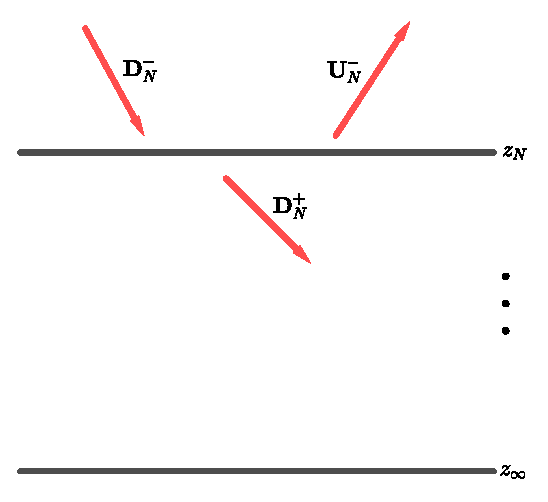
\includegraphics[scale=1]{ondas_em_zn}
\caption{\textit{Ondas ascendentes e descendentes na \'ultima interface. Observe que n\~ao h\'a ondas ascendentes depois da \'ultima camada}.}
\label{fig.ondas_em_zn}
\end{figure}

Substituindo a equa\c{c}\~ao \ref{eq.inversa_matriz_salto} na equa\c{c}\~ao anterior, temos
\begin{align*}
\begin{pmatrix}
\mathbf{U}_N^-\\
\mathbf{D}_N^-
\end{pmatrix}
&=
\begin{pmatrix}
J_{A,N}^\top&-J_{B,N}^\top\\
-J_{B,N}^\top&J_{A,N}^\top
\end{pmatrix}
\,
\begin{pmatrix}
0\\
\mathbf{D}_N^+
\end{pmatrix}\\\\
&=
\begin{pmatrix}
-J_{B,N}^\top \mathbf{D}_N^+\\
 J_{A,N}^\top \mathbf{D}_N^+
\end{pmatrix},
\end{align*}
ou seja,
\begin{align*}
\mathbf{U}_N^-&=-J_{B,N}^\top J_{A,N}^{-\top}\mathbf{D}_N^-\\
\mathbf{D}_N^+&=J_{A,N}^{-\top}\mathbf{D}_N^-.
\end{align*}
Assim, vemos que para computar uma onda refletida, ou seja, uma onda ascendente a partir de uma interface entre camadas, usamos uma \textit{matriz de reflex\~ao} que fica definida como
\begin{equation}\label{eq.reflexao_N}
\Gamma_N=-J_{B,N}^\top J_{A,N}^{-\top}.
\end{equation} 
Analogamente, vemos que para computar uma onda transmitida, ou seja, uma onda descendente a partir de uma interface entre camadas, usamos uma \textit{matriz de transmiss\~ao} que fica definida como
\begin{equation}\label{eq.transmissao_N}
T_N=J_{A,N}^{-\top}.
\end{equation} 

\subsubsection{Reflex\~ao e Transmiss\~ao numa Interface Qualquer}
Definimos a espessura de uma camada, a partir da interface superior, como
\begin{equation}
\Delta\,z_m=z_{m+1}-z_m,\qquad m=1,2,...,N-1,
\end{equation}
e temos que uma onda se propagando da interface na profundidade $z_m$ at\'e a interface em $z_{m+1}$ percorre uma profundidade total $\Delta\,z_m$. O valor dessa onda no fim da trajet\'oria, quando $z=z_{m+1}$, \'e aproximadamente igual a $\mathbf{\Psi}^-_{m+1}$, conforme a figura \ref{fig.N_interfaces}. Assim, usando a solu\c{c}\~ao \ref{eq.solucao_psi} podemos escrever
\begin{equation}\label{eq.solucao_delta_zm}
\mathbf{\Psi}^-_{m+1}=e^{-i\,\omega\tilde{\Lambda}_m\Delta\,z_m}\mathbf{\Psi}^+_m.
\end{equation}

\begin{figure}
\centering
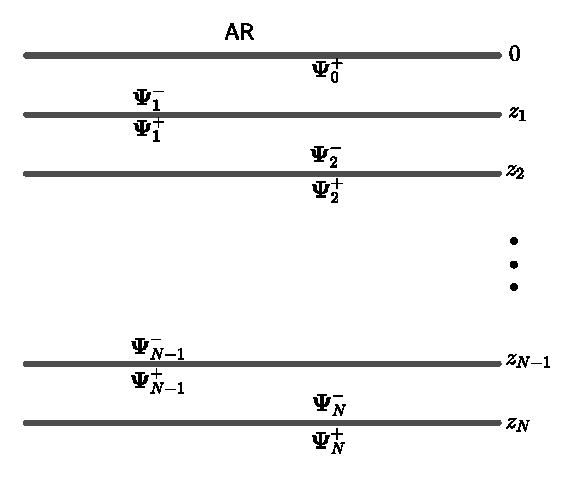
\includegraphics[scale=1]{n_interfaces}
\caption{\textit{Visualiza\c{c}\~ao de $N$ interfaces em subsuperf\'icie e a nota\c{c}\~ao das ondas nas proximadades de cada interface.}}
\label{fig.N_interfaces}
\end{figure}

Sabendo que essa onda se propagando na camada abaixo da interface em $z_m$ veio da camada anterior, podemos usar a matriz de salto na equa\c{c}\~ao \ref{eq.psi_matriz_salto} e escrever
\begin{align}\label{eq.salto_m}
\mathbf{\Psi}^+_{m}&=J_m\,\mathbf{\Psi}^-_m.
\end{align}
Substituindo a equa\c{c}\~ao \ref{eq.salto_m} na equa\c{c}\~ao \ref{eq.solucao_delta_zm}, temos
\begin{align}\label{eq.psi_m-}\nonumber
\mathbf{\Psi}^-_{m+1}&=e^{-i\,\omega\tilde{\Lambda}_m\Delta\,z_m}\mathbf{\Psi}^+_m\\\nonumber
\mathbf{\Psi}^-_{m+1}&=e^{-i\,\omega\tilde{\Lambda}_m\Delta\,z_m}J_m\,\mathbf{\Psi}^-_m\\
\mathbf{\Psi}^-_m&=J^{-1}_me^{i\,\omega\tilde{\Lambda}_m\Delta\,z_m}\mathbf{\Psi}^-_{m+1}
\end{align}
Substituindo a equa\c{c}\~ao \ref{eq.definicao_psi} e a equa\c{c}\~ao \ref{eq.inversa_matriz_salto} na equa\c{c}\~ao \ref{eq.psi_m-}, temos
\begin{align}\label{eq.refle_trans_1}
\mathbf{U}_m^-&=J^\top_{A,m}e^{i\,\omega\Lambda_m\Delta\,z_m}\mathbf{U}^-_{m+1}-J^\top_{B,m}e^{-i\,\omega\Lambda_m\Delta\,z_m}\mathbf{D}^-_{m+1}\\\nonumber\\\label{eq.refle_trans_2}
\mathbf{D}_m^-&=-J^\top_{B,m}e^{i\,\omega\Lambda_m\Delta\,z_m}\mathbf{U}^-_{m+1}+J^\top_{A,m}e^{-i\,\omega\Lambda_m\Delta\,z_m}\mathbf{D}^-_{m+1}.
\end{align}
Assim como definimos matriz de reflex\~ao para a \'ultima interface em $z_N$, podemos definir a matriz de reflex\~ao para uma interface qualquer, ou seja,
\begin{equation}\label{eq.reflexao_m+1}
\mathbf{U}^-_{m+1}=\Gamma_{m+1}\mathbf{D}^-_{m+1}.
\end{equation}
Substituindo a equa\c{c}\~ao \ref{eq.reflexao_m+1} na equa\c{c}\~ao \ref{eq.refle_trans_1} e na equa\c{c}\~ao \ref{eq.refle_trans_2}, temos
\begin{align}\label{eq.refle_trans_3}
\mathbf{U}_m^-&=(J^\top_{A,m}e^{i\,\omega\Lambda_m\Delta\,z_m}\Gamma_{m+1}-J^\top_{B,m}e^{-i\,\omega\Lambda_m\Delta\,z_m})\mathbf{D}^-_{m+1}\\\nonumber\\\label{eq.refle_trans_4}
\mathbf{D}_m^-&=(-J^\top_{B,m}e^{i\,\omega\Lambda_m\Delta\,z_m}\Gamma_{m+1}+J^\top_{A,m}e^{-i\,\omega\Lambda_m\Delta\,z_m})\mathbf{D}^-_{m+1}\,.
\end{align}
Substituindo a equa\c{c}\~ao \ref{eq.refle_trans_4} na equa\c{c}\~ao \ref{eq.refle_trans_3}, temos
\begin{align*}
\mathbf{U}_m^-&=(J^\top_{A,m}e^{i\,\omega\Lambda_m\Delta\,z_m}\Gamma_{m+1}-J^\top_{B,m}e^{-i\,\omega\Lambda_m\Delta\,z_m})\\
&\,\,\cdot\,\,(-J^\top_{B,m}e^{i\,\omega\Lambda_m\Delta\,z_m}\Gamma_{m+1}+J^\top_{A,m}e^{-i\,\omega\Lambda_m\Delta\,z_m})^{-1}\mathbf{D}_m^-\,,
\end{align*}
de onde podemos concluir que a matriz de reflex\~ao em uma interface em $z_m$ qualquer \'e dada por
\begin{align*}
\Gamma_{m}&=(J^\top_{A,m}e^{i\,\omega\Lambda_m\Delta\,z_m}\Gamma_{m+1}-J^\top_{B,m}e^{-i\,\omega\Lambda_m\Delta\,z_m})\\
&\,\,\cdot\,\,(-J^\top_{B,m}e^{i\,\omega\Lambda_m\Delta\,z_m}\Gamma_{m+1}+J^\top_{A,m}e^{-i\,\omega\Lambda_m\Delta\,z_m})^{-1},
\end{align*}
ou
\begin{align}\nonumber
\Gamma_{m}&=(J^\top_{A,m}e^{i\,\omega\Lambda_m\Delta\,z_m}\Gamma_{m+1}e^{i\,\omega\Lambda_m\Delta\,z_m}-J^\top_{B,m})\\\label{eq.matriz_reflexao_m}
&\,\,\cdot\,\,(-J^\top_{B,m}e^{i\,\omega\Lambda_m\Delta\,z_m}\Gamma_{m+1}e^{i\,\omega\Lambda_m\Delta\,z_m}+J^\top_{A,m})^{-1}.
\end{align}
Quando uma onda atinge uma interface, al\'em da possibilidade de reflex\~ao h\'a tamb\'em a possibilidade de trasmiss\~ao da onda para a camada inferior. De maneira an\'aloga ao desenvolvido para reflex\~ao de ondas, podemos deduzir a matriz para a transmiss\~ao de ondas em uma interface qualquer, que \'e dada por
\begin{equation}\label{eq.matriz_transmissao_m}
T_m=T_{m+1}e^{i\,\omega\,\Lambda\Delta\,z_m}(-J^\top_{B,m}e^{i\,\omega\Lambda_m\Delta\,z_m}\Gamma_{m+1}e^{i\,\omega\Lambda_m\Delta\,z_m}+J^\top_{A,m})^{-1}.
\end{equation}
A validade das equa\c{c}\~oes \ref{eq.matriz_reflexao_m} e \ref{eq.matriz_transmissao_m} para qualquer interface pode ser demonstrada por indu\c{c}\~ao sobre $m$, e todas as matrizes de reflex\~ao e transmiss\~ao podem ser computadas por recurss\~ao partindo das equa\c{c}\~oes \ref{eq.reflexao_N} e \ref{eq.transmissao_N}.

\section{Solu\c{c}\~ao na Presen\c{c}a de Fonte}\label{sec.presenca_fonte}
Em prospec\c{c}\~ao de petr\'oleo s\~ao utilizadas alguns tipos de fontes de ondas, atrav\'es das quais se faz um mapeamento das caracter\'isticas das camadas de subsuperf\'icie. Segundo \cite{dobrin_88}, esses tipos de fontes podem ser uma queda de peso, um caminh\~ao \textit{vibroseis}, explosivos e canh\~ao de ar, esta \'ultima fonte utilizada em prospec\c{c}\~ao mar\'itima. Sendo assim, vamos desenvolver uma solu\c{c}\~ao para o nosso problema considerando agora a presen\c{c}a de uma fonte.

Considere ainda a equa\c{c}\~ao \ref{eq.matricial} com o sobrescrito $m$ omitido. Uma fonte $\mathbf{S}$ localizada numa profundidade $z_s$ pode ser representada na forma
\begin{equation}\label{eq.fonte_geral}
\mathbf{S}=\mathbf{S}_0\delta(z-z_s)+\mathbf{S}_1\delta^\prime(z-z_s),
\end{equation}
onde $\mathbf{S}_0$ e $\mathbf{S}_1$ n\~ao dependem da profundidade e $\delta$ \'e a fun\c{c}\~ao \textit{Delta de Dirac} conforme a subse\c{c}\~ao \ref{sec.dirac}. Fontes que s\~ao distribu\'idas ao longo da profundidade podem, geralmente, ser sintetizadas por superposi\c{c}\~ao de fontes do tipo $\mathbf{S}_0$ e $\mathbf{S}_1$. 

Uma solu\c{c}\~ao por ser escrita como a combina\c{c}\~ao de uma solu\c{c}\~ao inicial sofrendo a a\c{c}\~ao de alguma fonte, ou seja,
\begin{equation}\label{eq.solucao_inicial_fonte}
\mathbf{\Phi}=\mathbf{\Phi}_0+\mathbf{S}_1\delta(z-z_s).
\end{equation} 
Substituindo a equa\c{c}\~ao \ref{eq.solucao_inicial_fonte} e a equa\c{c}\~ao \ref{eq.fonte_geral} na equa\c{c}\~ao \ref{eq.matricial}, temos
\begin{equation}\label{eq.matricial_fonte}
\frac{d\,\mathbf{\Phi}_0}{d\,z}=-i\,\omega\,M\,\mathbf{\Phi}_0+\left[\mathbf{S}_0-i\,\omega\,M\,\mathbf{S}_1\right]\,\delta(z-z_s),
\end{equation}
e por simplicidade, vamos escrever
\begin{equation}\label{eq.fonte_simplificada}
i\,\omega\,M\,\mathbf{S}_1-\mathbf{S}_0=
\begin{pmatrix}
\mathbf{S}_A\\
\mathbf{S}_B
\end{pmatrix}.
\end{equation}
Considerando a exist\^encia de uma interface imagin\'aria na profundidade $z_s$ da fonte, podemos determinar as condi\c{c}\~oes de salto no local da fonte da mesma forma que estudamos as condi\c{c}\~oes de salto nas interfaces que separam as camadas. Assim, integrando a equa\c{c}\~ao \ref{eq.matricial_fonte} no intervalo que come\c{c}a imediatamente acima da interface imagin\'aria da fonte $z_s^-$, e termina imediatamente abaixo da interface imagin\'aria da fonte em $z_s^+$, e substituindo a equa\c{c}\~ao \ref{eq.fonte_simplificada}, temos como solu\c{c}\~ao
\begin{equation*}
\mathbf{\Phi}_0(z_s^-)=\mathbf{\Phi}_0(z_s^+)+
\begin{pmatrix}
\mathbf{S}_A\\
\mathbf{S}_B
\end{pmatrix}.
\end{equation*}
Substituindo a equa\c{c}\~ao \ref{eq.solucao_inicial_fonte} e considerando as caracter\'isticas da fun\c{c}\~ao Delta de Dirac, temos a seguinte condi\c{c}\~ao de salto na profundidade da fonte
\begin{equation}\label{eq.salto_zs}
\mathbf{\Phi}(z_s^-)=\mathbf{\Phi}(z_s^+)+
\begin{pmatrix}
\mathbf{S}_A\\
\mathbf{S}_B
\end{pmatrix}.
\end{equation}

Vamos agora inserir uma interface imagin\'aria imediatamente abaixo da fonte, em $z=z_s^+$ e utilizar os m\'etodos do cap\'itulo \ref{sec.ausencia_fonte} para computar a matriz de reflex\~ao $\Gamma_s\equiv\Gamma(z_s^+)$ a partir do topo desta camada. J\'a que a interface em $z_s^+$ \'e fict\'icia, as propriedades do meio s\~ao iguais acima e abaixo dessa interface, assim temos que $L_2^+=L_2^-$ e $L_1^+=L_1^-$. Substituindo essas identidades nas equa\c{c}\~oes \ref{eq.j_a} e \ref{eq.j_b}, temos
\begin{align}\label{eq.j_a_ficticia}
J_A&=\frac{1}{2}\left[(L_2)^\top L_1+(L_1)^\top L_2\right]\\\label{eq.j_b_ficticia}
J_B&=\frac{1}{2}\left[(L_2)^\top L_1-(L_1)^\top L_2\right].
\end{align}
Substituindo as equa\c{c}\~oes \ref{eq.l1l2} e \ref{eq.l2l1} nas equa\c{c}\~oes \ref{eq.j_a_ficticia} e \ref{eq.j_b_ficticia}, obtemos que
\begin{align*}
J_A&=I\\
J_B&=0.
\end{align*}
Desta forma, a onda ascendente $\mathbf{U}(z_s^+)$ e a onda descendente $\mathbf{D}(z_s^+)$ a partir da interface em $z_s^+$ podem ser introduzidas na equa\c{c}\~ao \ref{eq.definicao_psi} para obtermos
\begin{equation*}
\mathbf{\Psi}(z_s^+)=
\begin{pmatrix}
\mathbf{U}(z_s^+)\\
\mathbf{D}(z_s^+)
\end{pmatrix}.
\end{equation*}
Substituindo a equa\c{c}\~ao \ref{eq.reflexao_m+1} na equa\c{c}\~ao acima, temos
\begin{equation}\label{eq.Psi_descendente}
\mathbf{\Psi}(z_s^+)=
\begin{pmatrix}
\Gamma_s\mathbf{D}(z_s^+)\\
\mathbf{D}(z_s^+)
\end{pmatrix},
\end{equation}
pois as ondas est\~ao numa mesma camada e da\'i usamos que
\begin{align*}
\mathbf{U}^-(z_s^+)&=\mathbf{U}(z_s^+)\\
\mathbf{D}^-(z_s^+)&=\mathbf{D}(z_s^+).
\end{align*}
Multiplicando a equa\c{c}\~ao \ref{eq.salto_zs} por $L^{-1}$ e substituindo a equa\c{c}\~ao \ref{eq.Phi}, obtemos
\begin{equation}\label{eq.Psi_salto_zs}
\mathbf{\Psi}(z_s^-)=\mathbf{\Psi}(z_s^+)+L^{-1}
\begin{pmatrix}
\mathbf{S}_A\\
\mathbf{S}_B
\end{pmatrix}.
\end{equation}
Substituindo a express\~ao para $L^{-1}$ dada pela equacao \ref{eq.L^-1}, juntamente com a equa\c{c}\~ao \ref{eq.Psi_descendente} na equa\c{c}\~ao \ref{eq.Psi_salto_zs}, temos
\begin{equation}\label{eq.solucao_phi_zs-}
\mathbf{\Psi}(z_s^-)=
\begin{pmatrix}
\Gamma_s\mathbf{D}(z_s^+)\\
\mathbf{D}(z_s^+)
\end{pmatrix}
+
\frac{1}{\sqrt{2}}\,
\begin{pmatrix}
L_2^\top\mathbf{S}_A+L_1^\top\mathbf{S}_B\\
L_2^\top\mathbf{S}_A-L_1^\top\mathbf{S}_B
\end{pmatrix}.
\end{equation}
Admitindo que a fonte esteja no interior da primeira camada, ou seja, $0<z_s<z_1$, a solu\c{c}\~ao dada pela equa\c{c}\~ao \ref{eq.solucao_phi_zs-} \'e propagada para cima a partir de $z_s^-$ usando a equa\c{c}\~ao \ref{eq.solucao_psi}, e o salto atrav\'es das interfaces entre camadas \'e dado pela equa\c{c}\~ao \ref{eq.psi_matriz_salto} at\'e que a onda atinja a interface terra/ar em $z=0^+$. Assim,
\begin{equation*}
\mathbf{\Psi}(0^+)=e^{-i\,\omega\,\tilde{\mathbf{\Lambda}}\,(0^+-z_s^-)}\,\mathbf{\Psi}(z_s^-),
\end{equation*}
e podemos usar as $n$ condi\c{c}\~oes de fronteira em $z=0$ para determinarmos as $n$ inc\'ognitas de $\mathbf{D}_s$. Os demais termos da solu\c{c}\~ao s\~ao conhecidos. A diferen\c{c}a $z_s^--0^+$ corresponde \`a profundidade da fonte, assim a solu\c{c}\~ao anterior pode ser reescrita como
\begin{align*}
\mathbf{\Psi}(0^+)&=e^{-i\,\omega\,\tilde{\mathbf{\Lambda}}\,(-z_s)}\,\mathbf{\Psi}(z_s^-)\\\\
\mathbf{\Psi}(0^+)&=
\begin{pmatrix}
e^{i\,\omega\,\mathbf{\Lambda}\,z_s}&\mathbf{0}\\
\mathbf{0}&e^{-i\,\omega\,\mathbf{\Lambda}\,z_s}
\end{pmatrix}
\mathbf{\Psi}(z_s^-).
\end{align*}
Substituindo a equa\c{c}\~ao \ref{eq.solucao_phi_zs-} na equa\c{c}\~ao acima, temos
\begin{equation}\label{eq.Psi_zero+}
\mathbf{\Psi}(0^+)=
\begin{pmatrix}
e^{i\,\omega\,\mathbf{\Lambda}\,z_s}\,\Gamma_s\mathbf{D}(z_s^+)\\
e^{-i\,\omega\,\mathbf{\Lambda}\,z_s}\,\mathbf{D}(z_s^+)
\end{pmatrix}
+
\frac{1}{\sqrt{2}}\,
\begin{pmatrix}
e^{i\,\omega\,\mathbf{\Lambda}\,z_s}\,(L_2^\top\mathbf{S}_A+L_1^\top\mathbf{S}_B)\\
e^{-i\,\omega\,\mathbf{\Lambda}\,z_s}\,(L_2^\top\mathbf{S}_A-L_1^\top\mathbf{S}_B)
\end{pmatrix},
\end{equation}
e teremos os valores de cada campo quando as ondas retornarem \`a superf\'icie.

